% tex/desenvolvimento/dev_02_pipeline_features.tex
\section{Pipeline de Engenharia de Features}
\label{sec:dev_pipeline_features}

\textbf{Definição:} \\
A transformação dos dados brutos multimodais em um formato numérico, denso e semanticamente rico é uma etapa fundamental e crítica em qualquer projeto de aprendizado de máquina. Para o MatchPredict-AI, o objetivo deste pipeline foi a criação de um vetor de características de alta dimensionalidade, especificamente com **2503 dimensões**, para cada um dos 2000 perfis. Este vetor robusto visa encapsular as múltiplas facetas de um perfil de usuário, desde sua aparência e auto-descrição textual até sua posição no ecossistema social de perfis. O processo completo está implementado em um conjunto de scripts modulares, principalmente `src/models/features.py`, `src/models/social_graph.py` e `src/models/combine_features.py`. A Figura \ref{fig:pipeline_dados_tcc2} ilustra o fluxo geral deste pipeline.

\begin{figure}[hbt]
    \centering
    % 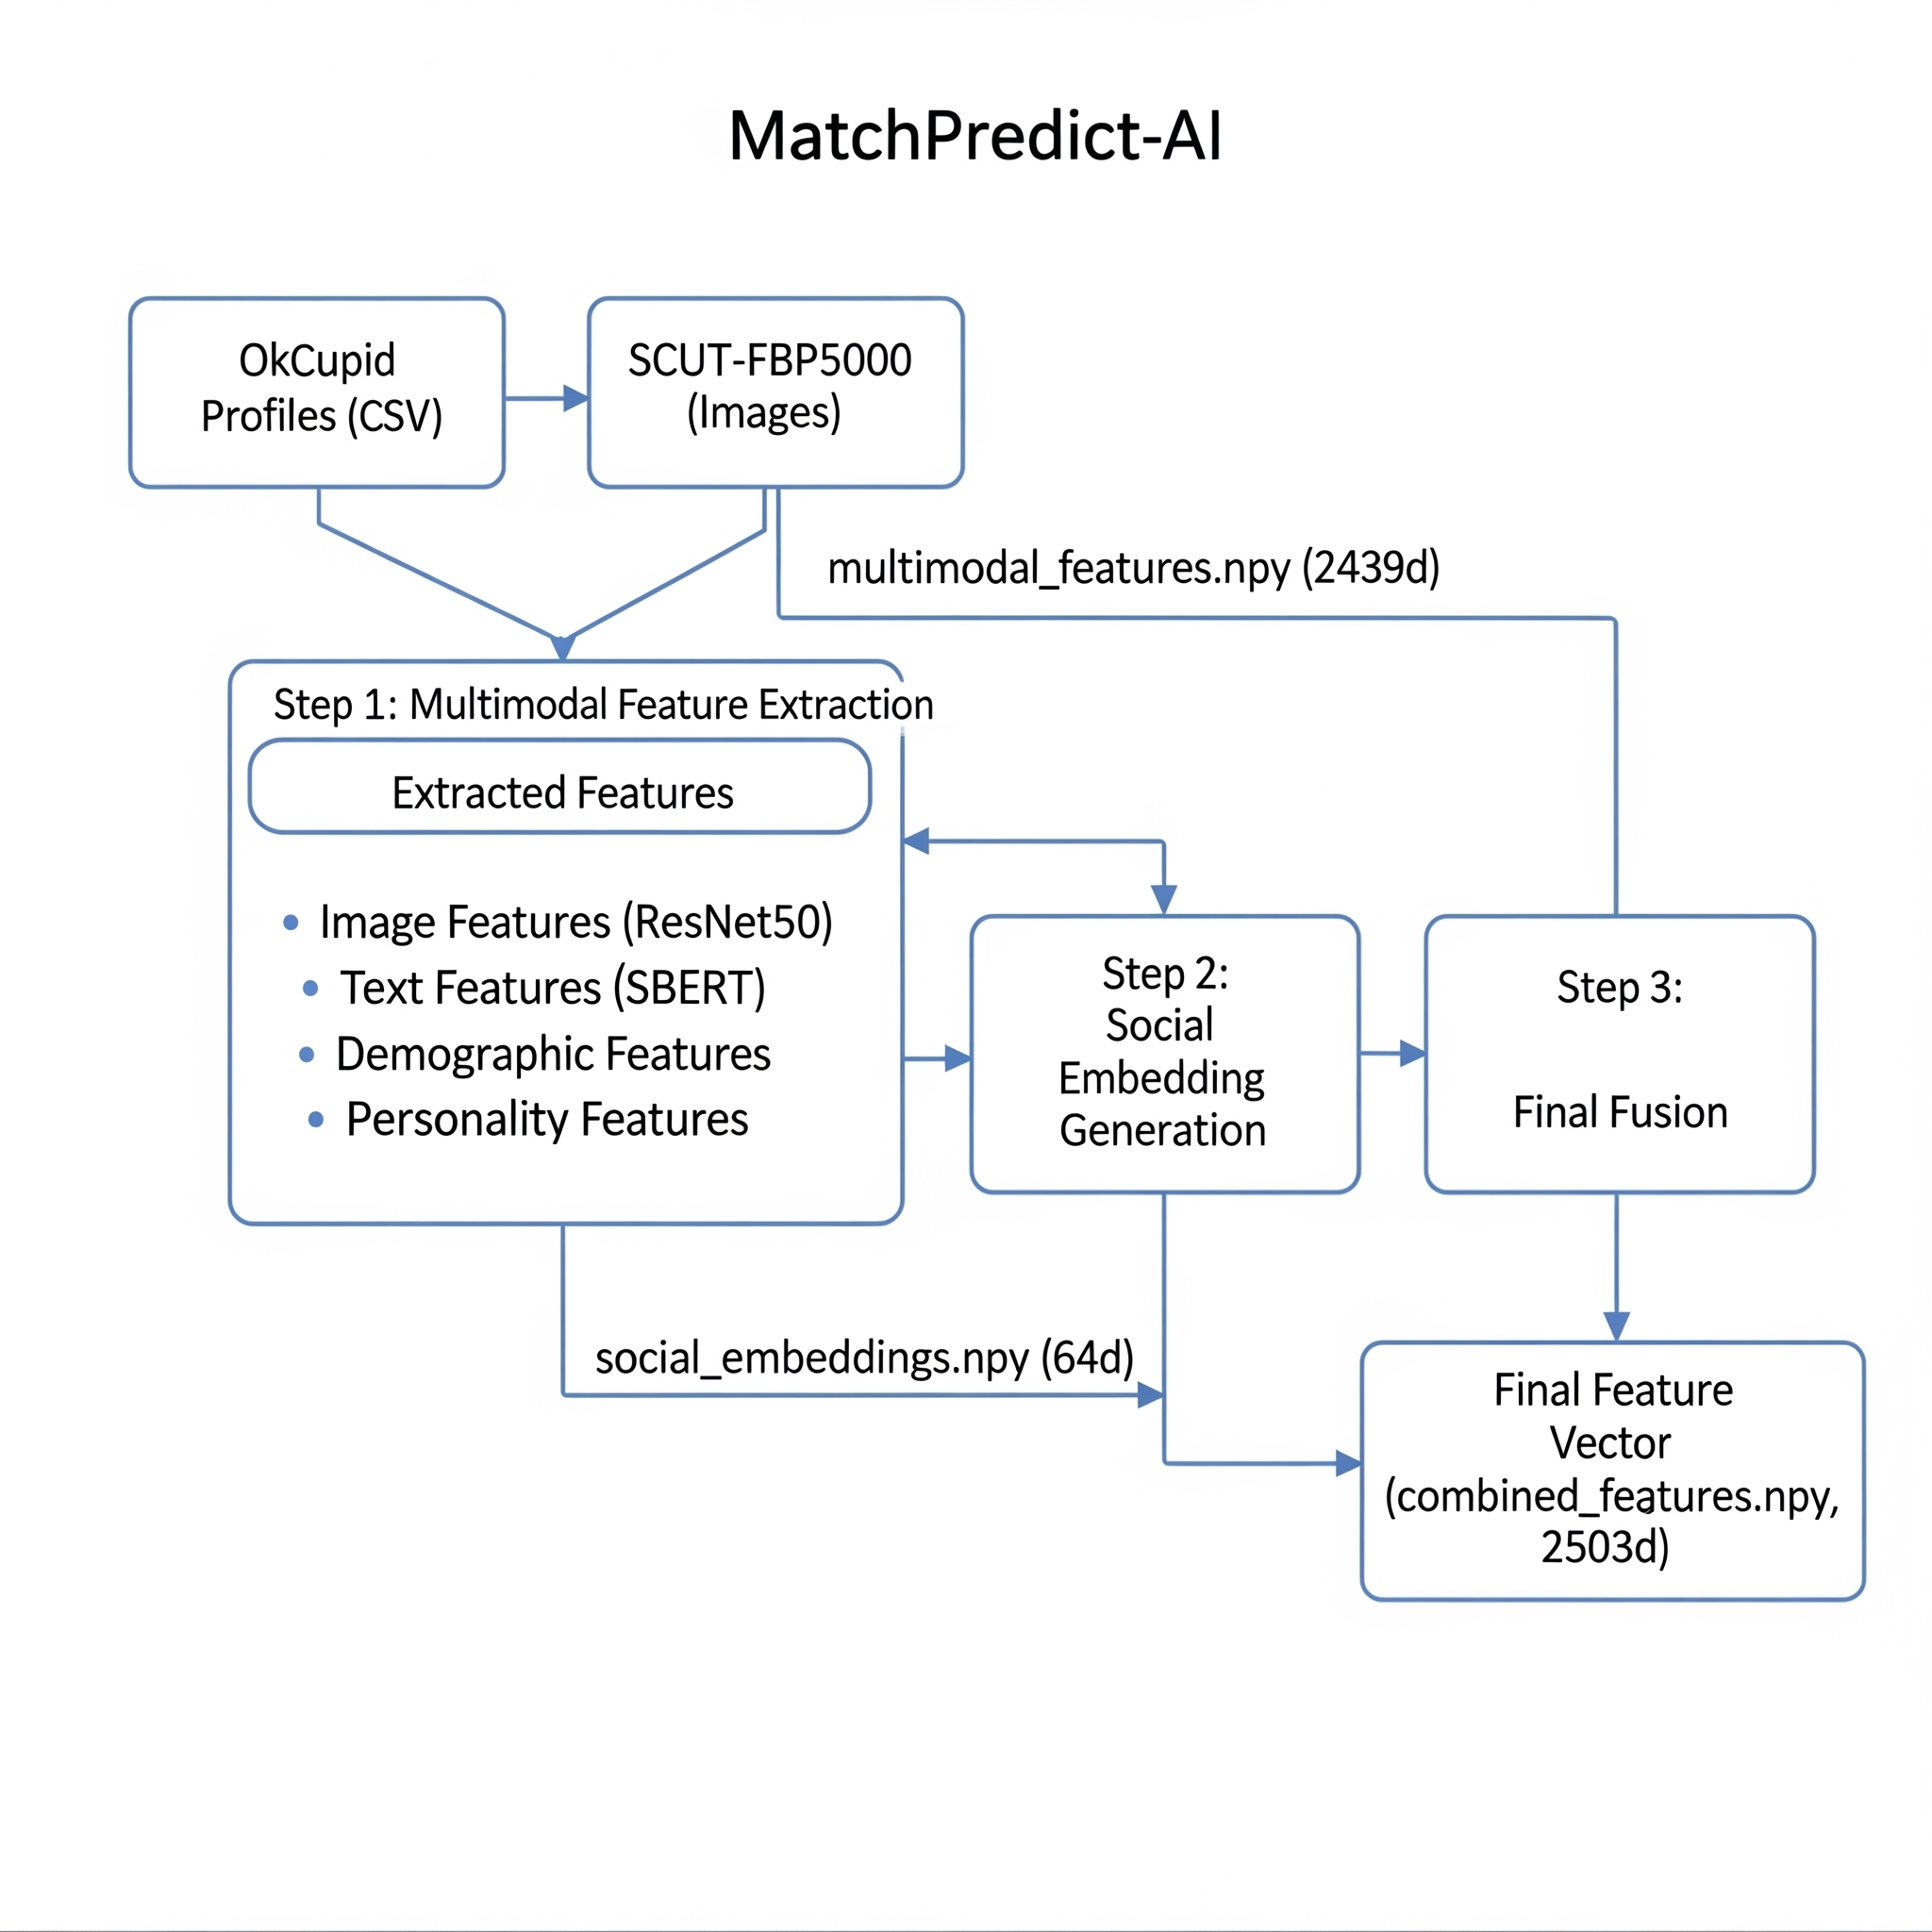
\includegraphics[width=\textwidth]{imagens/diagrama_pipeline.png} % Lembre-se de criar e adicionar esta imagem
    \framebox[0.9\textwidth][c]{\rule{0pt}{5cm} Espaço para o diagrama do pipeline de dados}
    \caption{Diagrama do pipeline de engenharia de features, ilustrando o fluxo desde os dados brutos até a composição do vetor final de 2503 dimensões.}
    \label{fig:pipeline_dados_tcc2}
\end{figure}

\subsection{Extração de Features Multimodais (2439 dimensões)}
\textbf{Implementação (`src/models/features.py`):} \\
A primeira fase do pipeline é responsável por processar as diferentes modalidades de dados (imagem, texto, etc.) e convertê-las em representações vetoriais.

\begin{itemize}
    \item \textbf{Features de Imagem (2048 dimensões):} As características visuais de cada perfil foram extraídas utilizando uma Rede Neural Convolucional (CNN) \textbf{ResNet50}, pré-treinada no vasto dataset ImageNet. A escolha da ResNet50 se deve ao seu reconhecido balanço entre profundidade arquitetural e capacidade de extrair features hierárquicas complexas. Em vez de usar a saída final do modelo, foi utilizado o vetor de ativação da penúltima camada (a camada de \textit{average pooling}), que resulta em um embedding de 2048 dimensões. Esta técnica de \textit{transfer learning} permite capturar características visuais abstratas e de alto nível (como formas, texturas e composições) que são mais úteis para tarefas de similaridade do que as classes finais da ImageNet.

    \item \textbf{Features de Texto (384 dimensões):} Para converter as biografias textuais (`essay0`) em vetores numéricos, foi empregado o modelo \textbf{Sentence-BERT}, especificamente a variante `all-MiniLM-L6-v2`. Esta arquitetura baseada em Transformers é projetada para gerar embeddings de sentenças que capturam o significado semântico do texto de forma contextualizada. O resultado é um vetor de 384 dimensões que representa a essência da auto-descrição do usuário, uma melhoria significativa sobre métodos mais antigos como Bag-of-Words, que ignoram o contexto e a semântica.

    \item \textbf{Features Demográficas (2 dimensões):} Dois dados demográficos foram incluídos: a idade, que foi normalizada para o intervalo [0, 1] para manter a consistência de escala com as outras features; e o sexo, que foi codificado numericamente (e.g., 0 para masculino, 1 para feminino).

    \item \textbf{Features de Personalidade (5 dimensões):} Para inferir traços de personalidade, foi implementado um método simples e eficaz baseado em léxico no script `src/models/personality.py`. Um dicionário de palavras-chave foi criado, associando termos a cada um dos cinco grandes traços de personalidade ("Big Five": Abertura, Conscienciosidade, Extroversão, Amabilidade e Neuroticismo). O texto da biografia de cada usuário é então escaneado, e a frequência normalizada de palavras de cada categoria gera um vetor de 5 dimensões. Este vetor serve como uma aproximação do perfil psicológico do usuário, baseada em como ele se descreve.
\end{itemize}
Ao final desta fase, o vetor multimodal de 2439 dimensões é salvo no arquivo `multimodal_features.npy`.

\subsection{Geração de Embeddings Sociais (64 dimensões)}
\textbf{Adaptação Metodológica:} \\
A proposta original do TCC1 considerava o uso de APIs de redes sociais (como a do Instagram) para construir um grafo social explícito, onde as arestas representariam amizades ou seguidores. Contudo, na prática, essa abordagem apresenta desafios significativos, como restrições de acesso a APIs, questões de privacidade do usuário e a dificuldade de mapear identidades entre diferentes plataformas. Para superar essa barreira, foi adotada uma solução alternativa, implementada em `src/models/social_graph.py`: a criação de um **grafo social implícito**, baseado na similaridade entre os próprios perfis do nosso dataset. Esta abordagem é metodologicamente robusta, autocontida e define "conexões sociais" como uma alta afinidade de características entre os perfis.

\textbf{Implementação (`src/models/social_graph.py`):}
\begin{enumerate}
    \item \textbf{Construção do Grafo de Similaridade:} Primeiramente, um grafo não-direcionado foi construído, onde os 2000 perfis do nosso dataset são os nós. Para criar as arestas, foi utilizado o algoritmo **K-Nearest Neighbors (KNN)**. Para cada perfil (nó), foram identificados os seus $k=10$ vizinhos mais próximos no espaço de features de 2439 dimensões. A métrica de proximidade utilizada foi a **similaridade de cosseno**, que é eficaz para medir a semelhança entre vetores de alta dimensionalidade. O resultado é um grafo onde as arestas conectam perfis que são muito parecidos em termos de imagem, texto, demografia e personalidade.
    \item \textbf{Aprendizado de Representação com Node2Vec:} Com o grafo de similaridade construído, o passo seguinte foi aprender uma representação vetorial (embedding) para cada nó que capturasse a topologia do grafo. Para isso, foi utilizado o algoritmo \textbf{Node2Vec}. Este algoritmo realiza "caminhadas aleatórias" (random walks) no grafo para gerar sequências de nós. Em seguida, ele aplica um modelo da família Word2Vec (especificamente, Skip-Gram) sobre essas sequências para aprender um embedding de baixa dimensionalidade -- neste caso, 64 dimensões -- para cada nó. O vetor resultante para um perfil não descreve mais suas características intrínsecas, mas sim sua **posição e papel estrutural dentro da rede de perfis similares**.
\end{enumerate}
Este processo, que culmina na criação do arquivo `social_embeddings.npy`, é fundamental para o componente `ItemModel` da arquitetura GraphRec.

\subsection{Fusão Final do Vetor de Features}
\textbf{Implementação (`src/models/combine_features.py`):} \\
A etapa final do pipeline é a simples, porém crucial, concatenação dos vetores de features gerados nas fases anteriores. O vetor multimodal de 2439 dimensões (`multimodal_features.npy`) e o vetor de embedding social de 64 dimensões (`social_embeddings.npy`) são combinados horizontalmente. O resultado é o vetor final de **2503 dimensões**, salvo no arquivo `combined_features.npy`, que servirá como a representação completa e rica de cada perfil para o modelo de recomendação.